\documentclass[12pt,fleqn,a4paper,oneside]{mybook} %Final!!!
%\documentclass[11pt,fleqn,a4paper,draft]{mybook} %DRAFT - highlights overflow, leaves out images

%\usepackage{microtype}
\usepackage[slovak]{babel}
\usepackage[utf8]{inputenc}
\usepackage[T1]{fontenc}
\usepackage[normalem]{ulem}
\usepackage{mathtools}  					
\usepackage{graphicx}
\usepackage{subfigure}
\usepackage{enumerate}
\usepackage{etoolbox}                       %Problematic URL in reference
\apptocmd{\sloppy}{\hbadness 10000\relax}{}{}%Removes badness warnings
%This is to remove warnings resulting by otherwise OK URL's
\usepackage[hyphens]{url}
\usepackage{notes}
\usepackage{indentfirst}






%This custom command defines how the literal menus look like.
\newcommand{\gui}[1]{{\emph{#1}}} %Gui commands, icon names, buttons
 % All code, functions, variables are typed like this
\newcommand{\code}[1]{{\lstinline[columns=fixed]{#1}}}

\newcommand{\angl}[1]{{\footnote{\emph{angl.}\ {#1}}}} %Shorthand english equivalent


\usepackage[left=25mm,right=25mm,top=25mm,bottom=25mm,paperwidth=210mm,paperheight=297mm,includehead]{geometry}

\usepackage{titlesec}
\titleformat{\chapter}[hang]{\normalfont\huge\bfseries}{\thechapter}{1em}{}


\DeclarePairedDelimiter{\diagpars}{(}{)}
\newcommand{\diag}{\operatorname{diag}\diagpars}

\let\oldhat\hat
\renewcommand{\vec}[1]{\boldsymbol{\mathbf{#1}}}
%\renewcommand{\hat}[1]{\oldhat{\boldsymbol{\mathbf{#1}}}}


\usepackage{amsthm}
\usepackage{etoolbox}% http://ctan.org/pkg/etoolbo
\theoremstyle{definition}
\newtheorem{exmp}{Pr\'{i}klad}[chapter]
\AtEndEnvironment{exmp}{\null\hfill\qedsymbol}

\usepackage{listings,color} 			    %To list Matlab code
\definecolor{mygrey}{gray}{0.5}	        %Define a gray color
\lstset{
basicstyle=\ttfamily,
numbers=none,
commentstyle=\color{mygrey},
breaklines=true,
}
%extended Matlab language
\lstdefinelanguage{exMatlab}[]{Matlab}      %Defining expanded Matlab
{morekeywords={rng,pyulear,plot,hold,randn,filter,length,abs,periodogram,fft,sin,randn,xcorr,fminsearch,dlqr,predmodelqp,dlyap,ones,linprog,quadprog,optimset,qpOASES,qpOASES_sequence,sysStruct,probStruct,mpt_control,volume,hull,extreme,mpt_exportc,mpt_getInput,sdpvar,blkdiag,sdpsettings,solvesdp,geomean,double},
sensitive=true,
alsoletter={_}
}



\pagestyle{empty}

\begin{document}
%%%%%%% Zaciaatok %%%%%%%%
\renewcommand\thepage{\roman{page}}
\pagenumbering{roman}
\thispagestyle{empty}

\noindent \begin{center}
\textbf{{\large{}SLOVENSKÁ TECHNICKÁ UNIVERZITA V BRATISLAVE}}\\
\textbf{{\large{}STROJNÍCKA FAKULTA}}\textbf{\large{} }\\
\vspace{3cm}
\par\end{center}

\noindent \begin{center}
\vspace{3cm}
\par\end{center}



\begin{center}
\textbf{\textsc{\Large{}AeroShield: Miniatúrny experimentálny modul aerokyvadla}}\\
\par\end{center}{\Large \par}

\begin{center}
\textbf{\large{}Bakalárska práca}\\
\par\end{center}{\large \par}

\begin{center}
{\large{}SjF-číslo b. práce}\\
\par\end{center}{\large \par}



\vfill
\noindent \textbf{\large{}2022} \hfill \textbf{\large{} Peter Tibenský}
\cleardoublepage

%%%%%% \chapter*{Predhovor}
\thispagestyle{empty}

Myslel som si že ma táto téma bude baviť. Až pokial som si neuvedomil, že to nebude až také jednoduché... 

Už od malička ma fascinovala elektronika a všetko čo sa vedelo pohybovať a ja som to vedel riadiť. Volba tejto bakalárskej práce preto bola jasnou voľbou. 

\cleardoublepage

 %%%%%%
\tableofcontents
\thispagestyle{empty}
\cleardoublepage

%%%%%% Jednotlive kapitoly %%%%%%%%%
\pagestyle{plain}
\pagenumbering{arabic}
\setcounter{page}{1}


\chapter*{Úvod}
\label{UVOD}
\addcontentsline{toc}{chapter}{Úvod}

    Tento dokument popisuje tvorbu, kód a funkcie stránky s názvom "SF", podľa iniciálov klienta. Táto stránka bola vytvorená
ako záverečný projekt k predmetu Databázy a internet. Stránka funguje ako akýsi online životopis kde si klient môže zadávať svoje pracovné texty, fotky, pdf súbory a iné.

Klient môže obsah stránky upravovať pomocou konta administrátora ktoré je zabezpečené pomocou mena a hesla. Ostatní užívatelia stránky si môžu jednotlivé podstránky iba prezerať. Administrátor má možnosť registrácie nových administrátorov, ktorý budú mať taktiež povolený prístup ku spraovaniu obsahu stránky. Strána vznikala priamo podľa požiadaviek klienta a boli do nej zapracované všetky žiadosti klienta.

V dokumentácii je podrobne popísané fungovanie stránky a všetky jej aspekty. Stránka vznikla za účelom splnenia podmienok hodnotenia predmetu Databázy a internet a za tým účelom boli na fungovanie použité všetky programovacie jazyky ktoré sme sa počas semestra naučili a to menovite:

\begin{itemize}
\item HTML (HyperText Markup Language) - jazyk použitý na základnú obsahovú štruktúru stránky,
\item PHP (PHP: Hypertext Preprocessor) - použitý na získavanie dynamických údajov zo stránky,
\item SQL (Structured Query Language) - použitý na vytvorenie a komunikáciu s databázami na MySQL serveri,
\item CSS (Cascading Style Sheets) - použitý na vizuálnu štrukturáciu stránky.
\end{itemize}


\chapter{Vizuál stránky}

Úvodná stránka index.php ktorá je jednoduchého designu, s Headerom\footnote[1]{Element <header> HTML predstavuje úvodný obsah, zvyčajne skupinu úvodných alebo navigačných pomôcok. Môže obsahovať niektoré prvky záhlavia, ale aj logo, vyhľadávací formulár, meno autora a ďalšie prvky.}, ktorý sa opakuje na každej podstránke, nás privíta krátkym textom ktorý momentálne nahrádza text Lorem Ipsum. Stránka má v Headery umiestnené logo SF ktoré je viditeľné aj v náhľade stránky, v lište prehliadača. Toto logo funguje taktiež ako odkaz, ktorý nás pri kliknutí, vždy premiestni na úvodnú stránku index.php. V spodnej časti stránky sú umiestnené 2 hypertextové odkazy na LinkedIn a email. Úvodnú stránku môžeme vidieť na obr.\ref{OBRAZOK 1.1}

\begin{figure}[!tbh]
\centering
\setlength{\fboxsep}{0pt}%
\setlength{\fboxrule}{1pt}%
\fbox{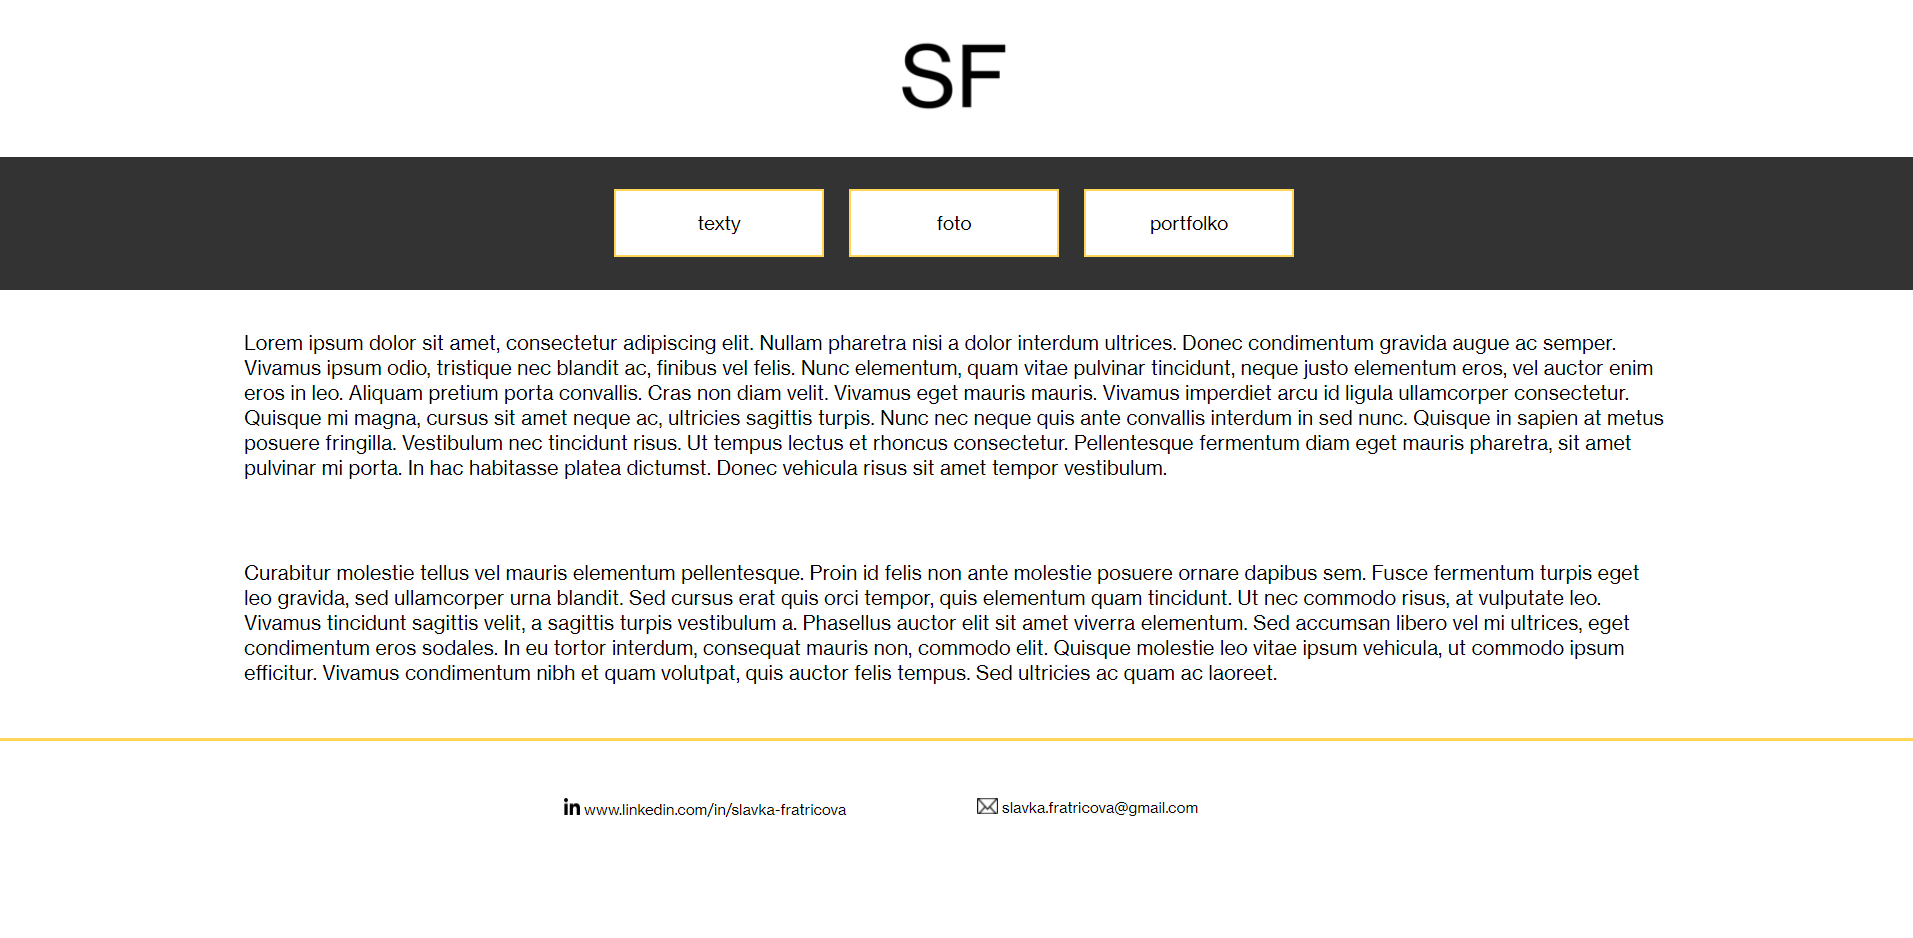
\includegraphics[width=\textwidth]{obr/uvodka.png}}
\caption{Úvodná stránka index.php.}\label{OBRAZOK 1.1}
\end{figure}








V časti texty, na podstránke indexx.php, nájde užívateľ nadpis a dátum publikácie článkov obr.\ref{OBRAZOK 1.2}. Po kliknutí na nadpis, sa užívateľovi zobrazí len požadovaný článok, ktorý sa rozvynie a zobrazí v celej dĺžke obr.\ref{OBRAZOK 1.3}.

\begin{figure}[!tbh]
\centering
\setlength{\fboxsep}{0pt}%
\setlength{\fboxrule}{1pt}%
\fbox{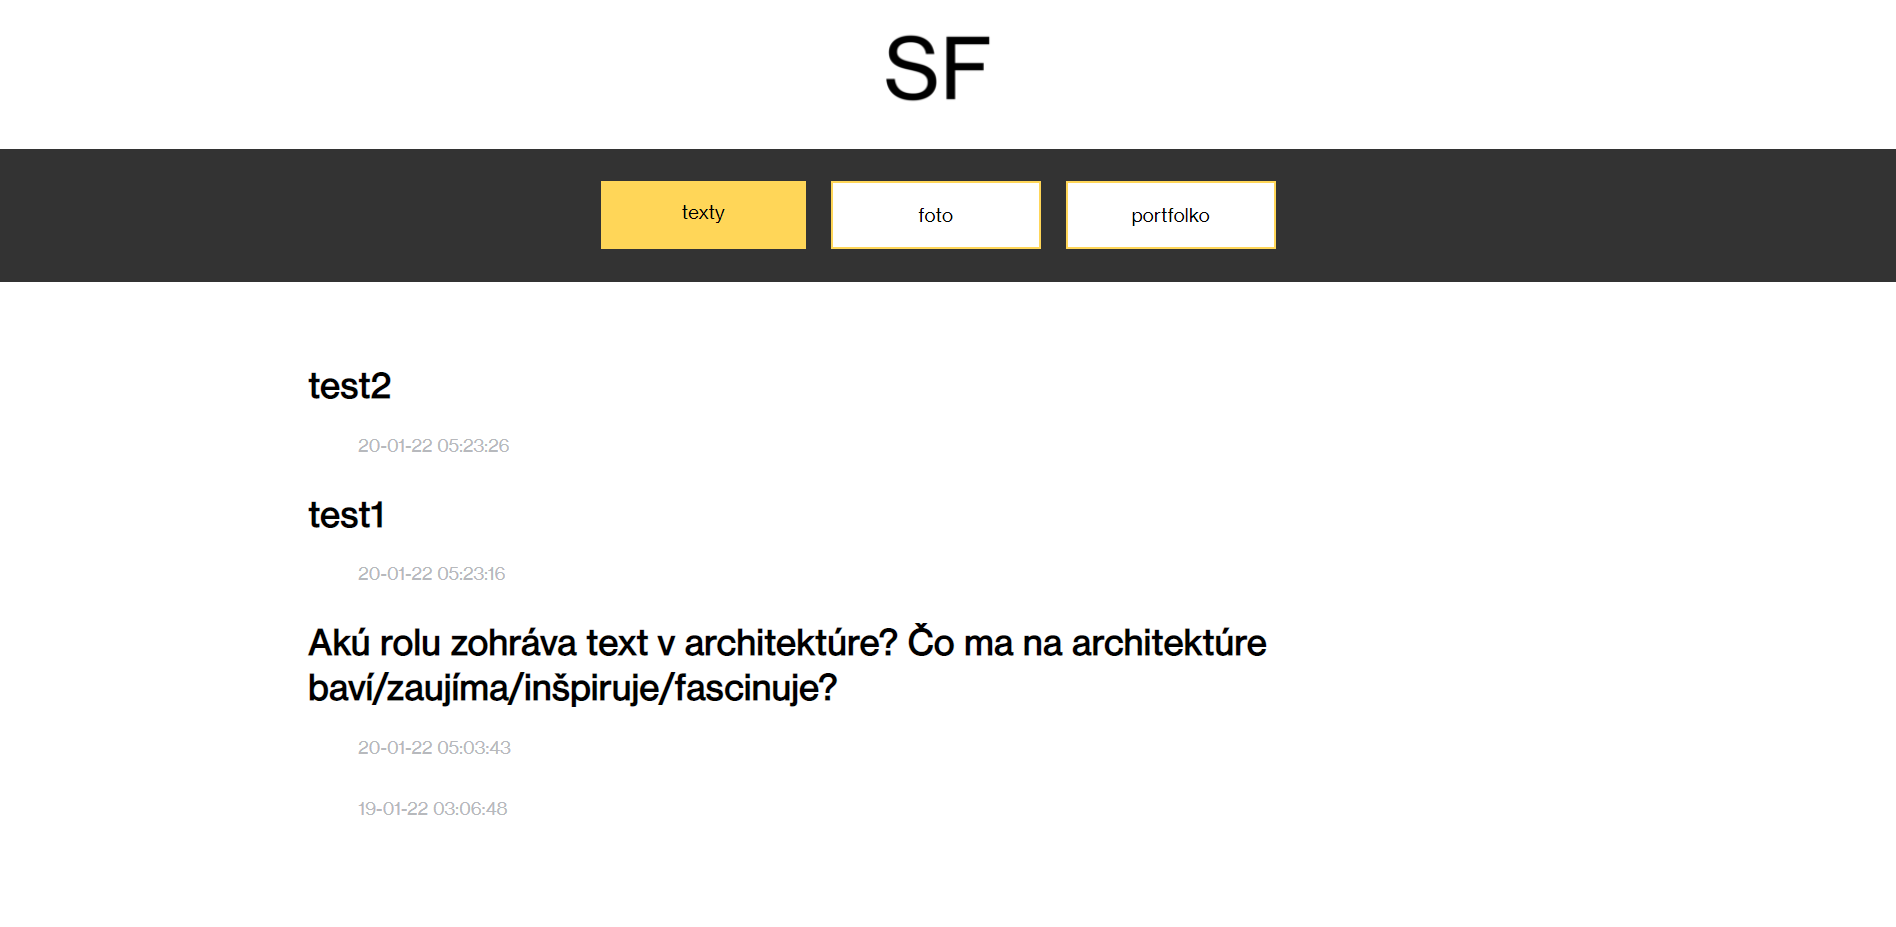
\includegraphics[width=\textwidth]{obr/texty_bez_text.png}}
\caption{Texty publikované na podstránke indexx.php.}\label{OBRAZOK 1.2}
\end{figure}

\begin{figure}[!tbh]
\centering
\setlength{\fboxsep}{0pt}%
\setlength{\fboxrule}{1pt}%
\fbox{
\includegraphics[width=\textwidth]{obr/texty_s_text.png}}
\caption{Zobrazenie konkrétneho textu na podstránke indexx.php.}\label{OBRAZOK 1.3}
\end{figure}

\vspace{5cm}

V časti foto nájde užívateľ výber fotiek, ktoré sa klient rozhodol zdieľať obr.\ref{OBRAZOK 1.4}. Fotky sú uložené v radoch, po troch fotkách, a pri prejdení kurzorom nad fotku, sa užívaťeľový zobrazí popis fotky obr.\ref{OBRAZOK 1.5}. Pri následnom kliknutí na fotku, sa konkrétna fotka maximalizuje(sú ale určené max. hodnoty šírky) a zobrazí sa aj príslušný nadpis a popis fotky obr.\ref{OBRAZOK 1.6}. Zobrazenie galérie ako aj fotky v okne je vykonávané pomocou java script kódu, využitého z open-source\footnote[2]{Open-source je zo všeobecného pohľadu akákoľvek informácia ktorá je dostupná verejnosti bez poplatku(s voľným prístupom), s ohľadom na fakt, že jej voľné šírenie zostane zachované.} projektu\cite{Gallery} .

\begin{figure}[!tbh]
\centering
\setlength{\fboxsep}{0pt}%
\setlength{\fboxrule}{1pt}%
\fbox{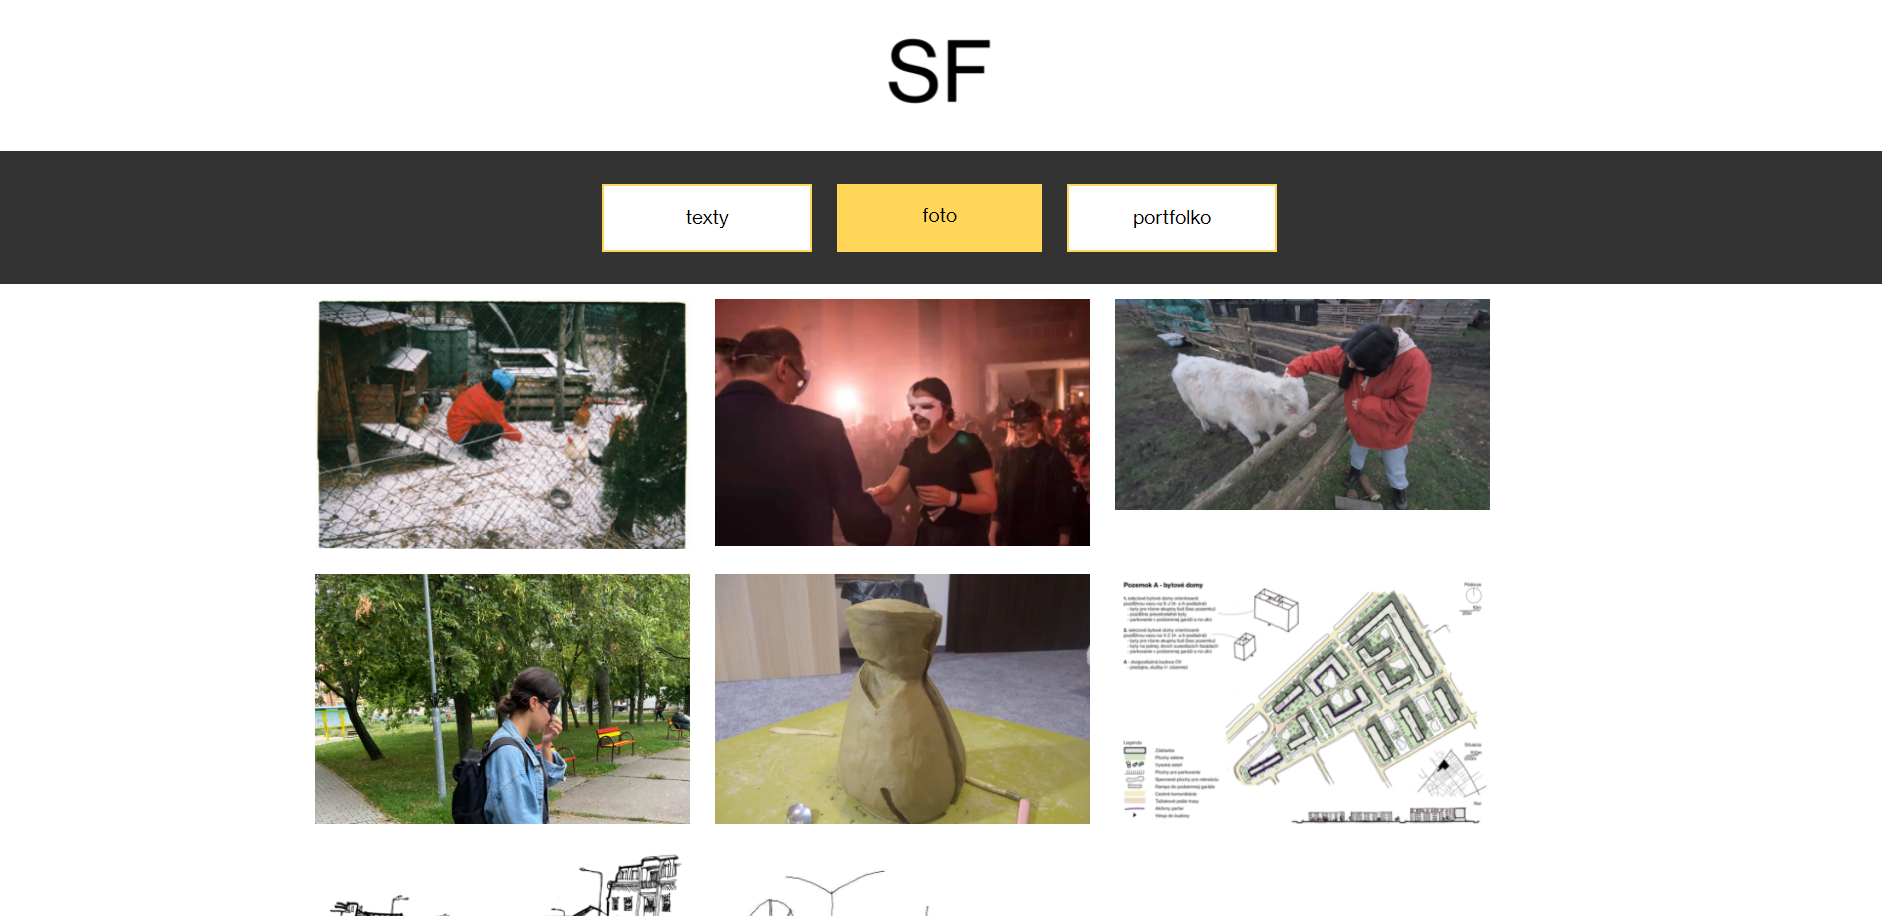
\includegraphics[width=\textwidth]{obr/galeria.png}}
\caption{Fotky publikované na podstránke foto.php.}\label{OBRAZOK 1.4}
\end{figure}

\begin{figure}[!tbh]
\centering
\setlength{\fboxsep}{0pt}%
\setlength{\fboxrule}{1pt}%
\fbox{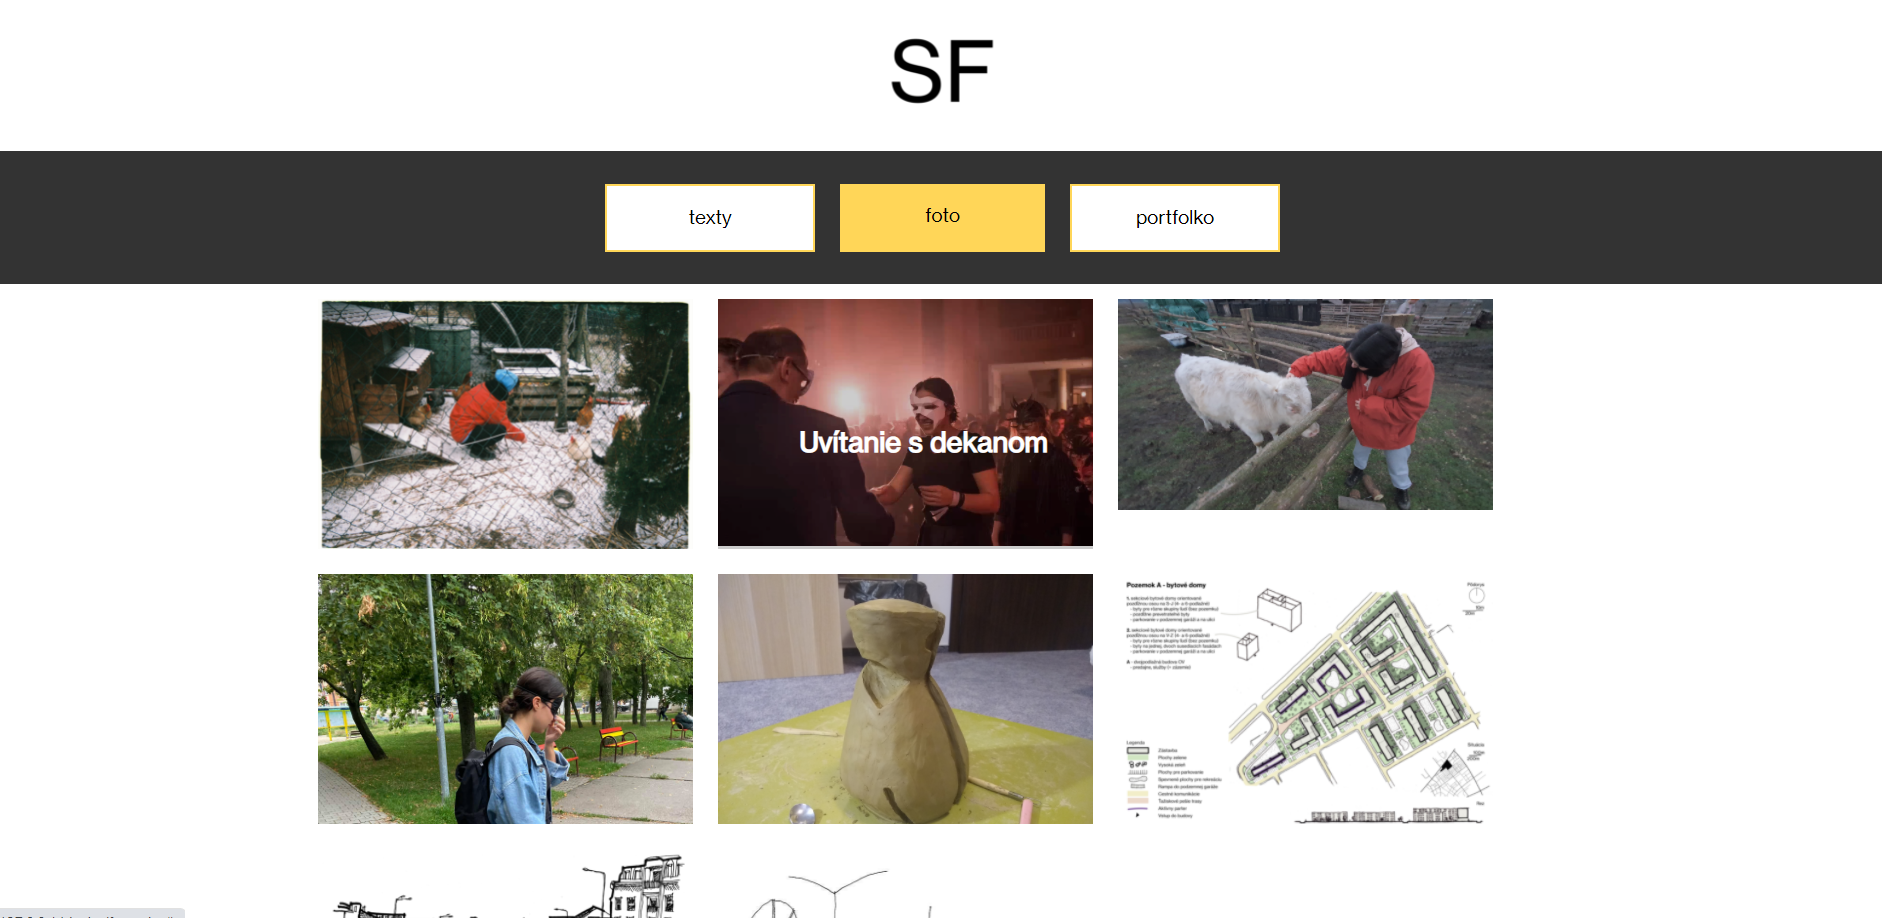
\includegraphics[width=\textwidth]{obr/galeria_nahlad.png}}
\caption{Náhlad popisu fotky na podstránke foto.php.}\label{OBRAZOK 1.5}
\end{figure}

\begin{figure}[!tbh]
\centering
\setlength{\fboxsep}{0pt}%
\setlength{\fboxrule}{1pt}%
\fbox{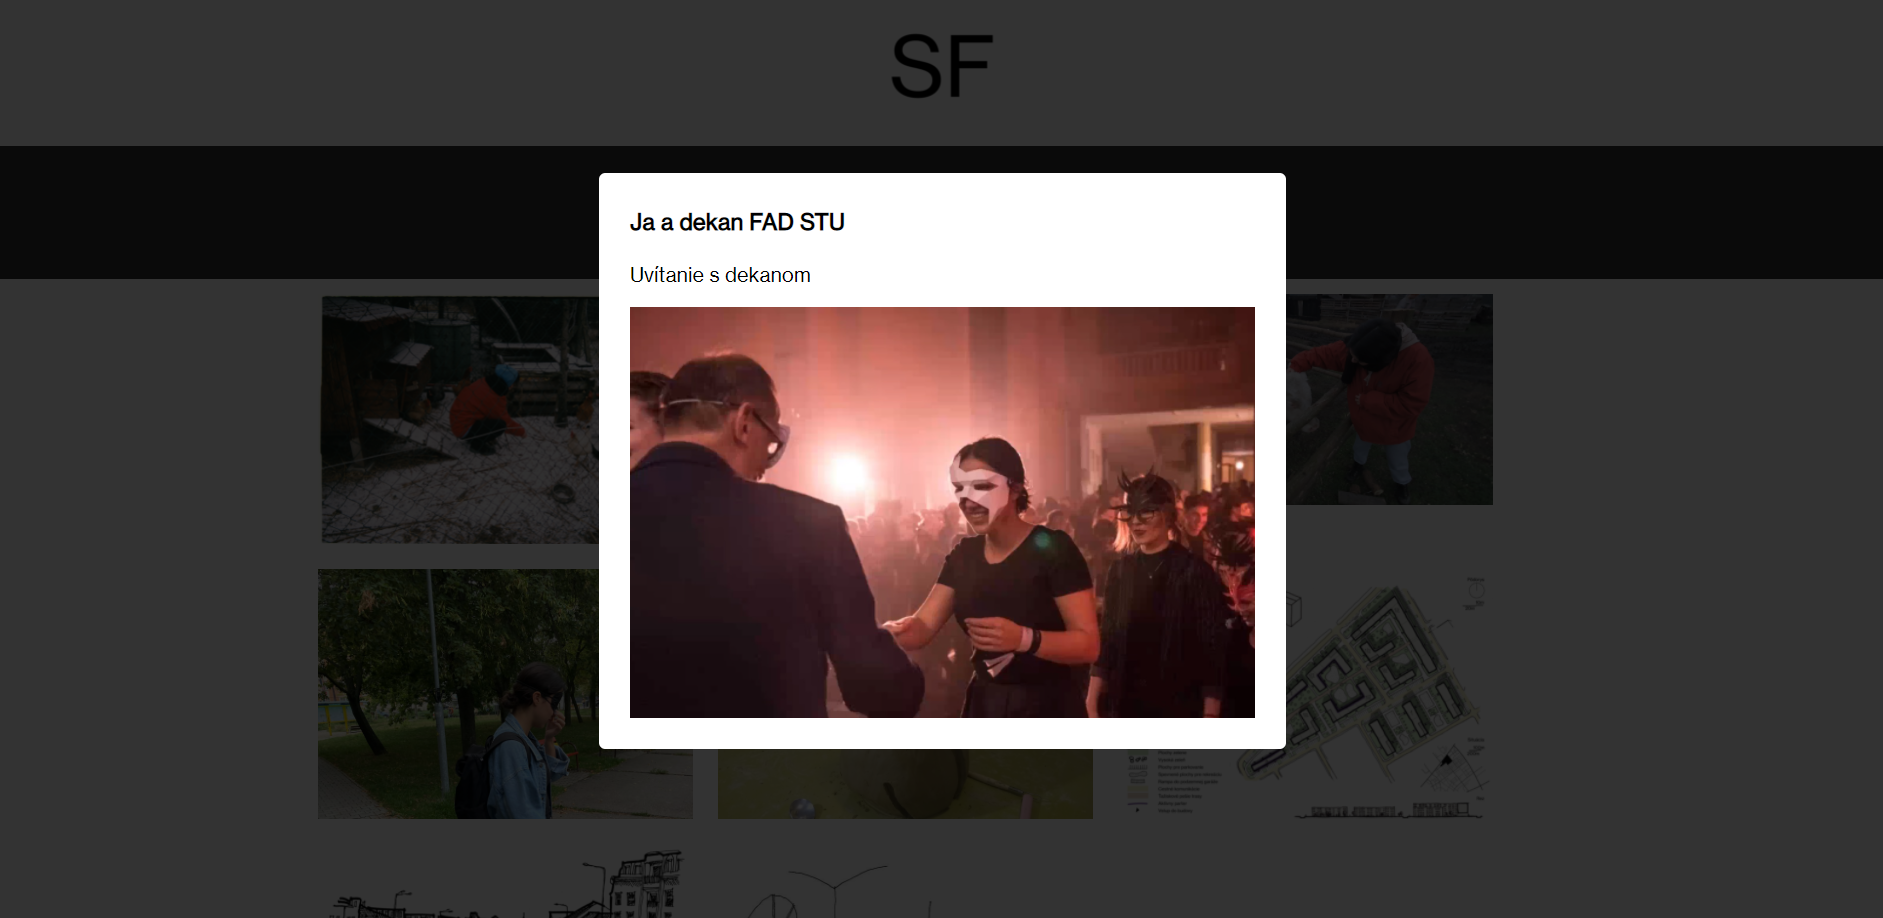
\includegraphics[width=\textwidth]{obr/galeria_zobrazenie.png}}
\caption{Zobrazenie konkrétnej fotky na podstránke foto.php.}\label{OBRAZOK 1.6}
\end{figure}


V časti portfolko, na podstránke portfolio.php, nájde užívateľ jednoduché okno v ktorom sa zobrazuje PDF súbor portfólia klienta obr.\ref{OBRAZOK 1.7}. Užívateľ si môže PDF súbor prezerať, alebo stiahnúť priamo zo stránky.

\begin{figure}[!tbh]
\centering
\setlength{\fboxsep}{0pt}%
\setlength{\fboxrule}{1pt}%
\fbox{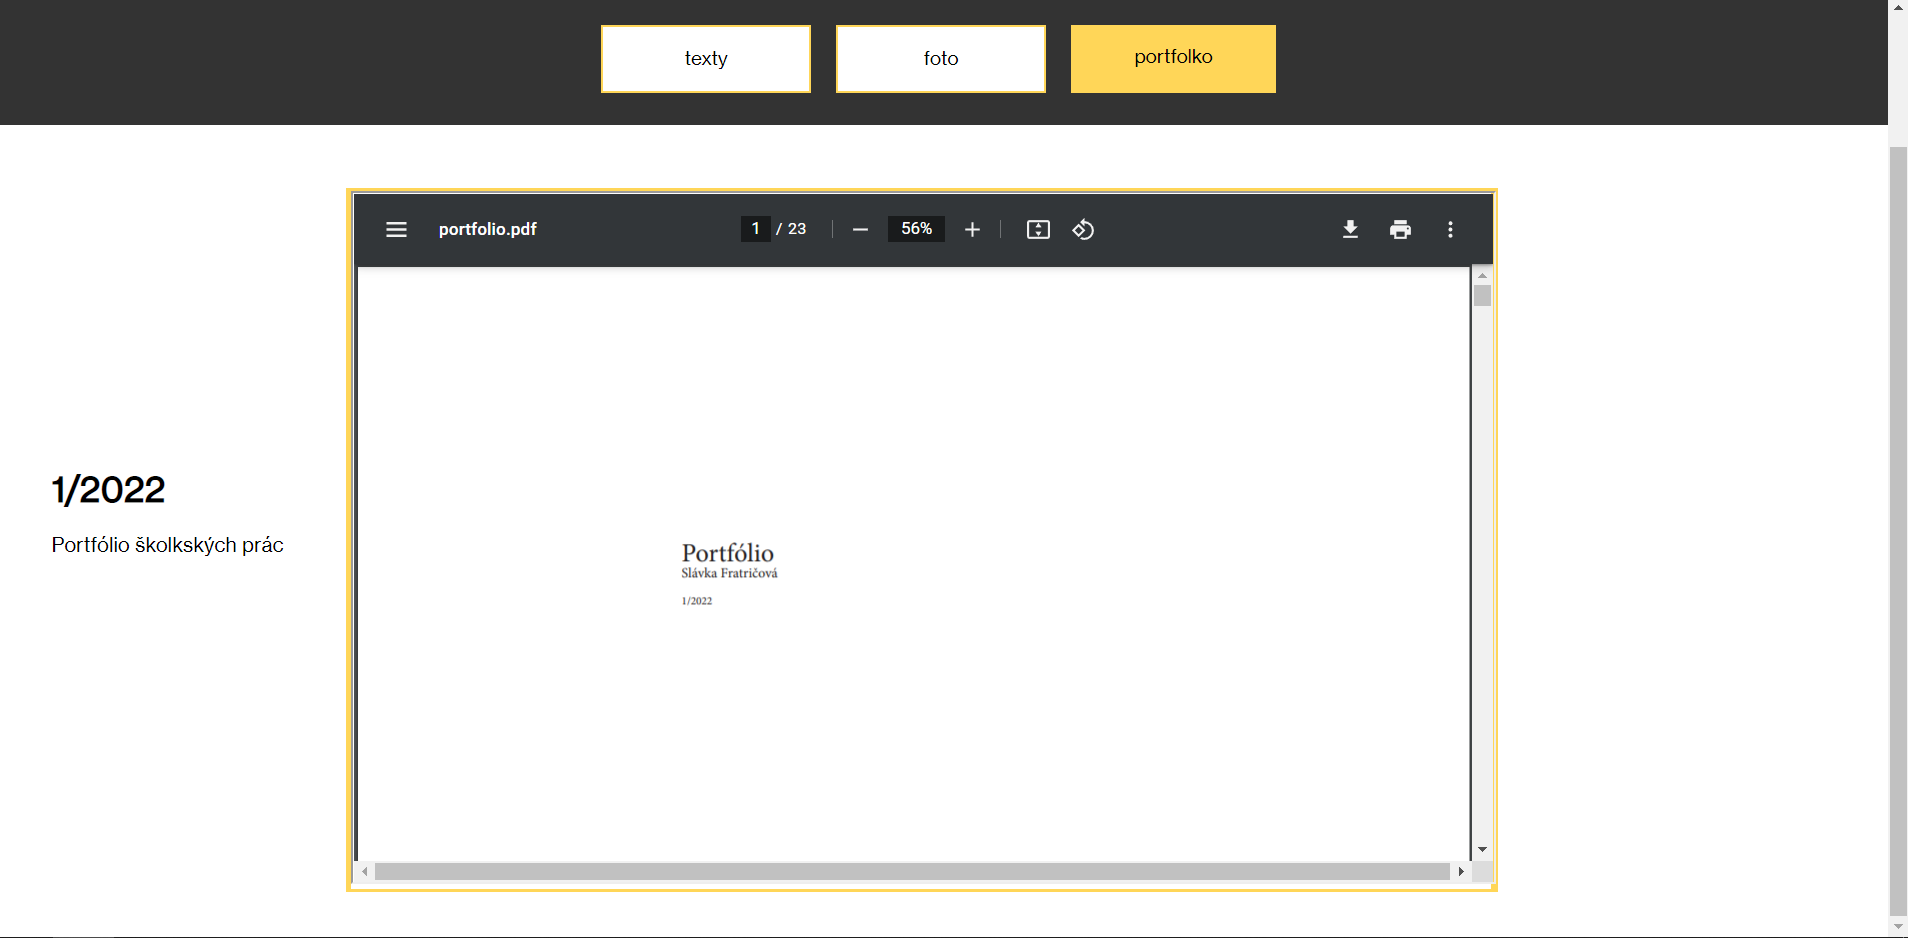
\includegraphics[width=\textwidth]{obr/portfolko.png}}
\caption{Portfólio na podstránke portfolio.php.}\label{OBRAZOK 1.7}
\end{figure}






\include{Funkcie stránky}
\include{Fungovanie stránky}
\chapter{Záver}

Táto časť diplomovej práce je povinná. Autor práce uvedie zhodnotenie riešenia, jeho výhody resp. nevýhody, použitie výsledkov, ďalšie možnosti a podobne.  Môže aj načrtnúť iný spôsob riešenia úloh, resp. uvedie, prečo postupoval uvedeným spôsobom.



%%%%%%% Koniec %%%%%%%%
\bibliographystyle{plain}
\addcontentsline{toc}{chapter}{Literat\'{u}ra}
\bibliography{bibliog}
\end{document}
